\documentclass{article}
\usepackage{listings}
\usepackage{xcolor}
\usepackage{graphicx}
\usepackage[a4paper, margin=1in]{geometry}
\setlength{\parindent}{0pt}

\title{Week5 Lab2 Report}
\author{111062117, Hsiang-Sheng Huang}

\begin{document}

\maketitle

\section*{Q1}
% Determine the installation location of Samtools. Demonstrate a method to locate it, without using information from the spack install output.
\begin{lstlisting}[language=bash, basicstyle=\ttfamily\small, numbers=left, numberstyle=\tiny\color{gray}, stepnumber=1, frame=single, breaklines=true, breakatwhitespace=false]
$ spack load samtools@1.19.2
$ which samtools
\end{lstlisting}

The output will show the path to the Samtools executable.
\begin{lstlisting}[language=bash, basicstyle=\ttfamily\small, numbers=left, numberstyle=\tiny\color{gray}, stepnumber=1, frame=single, breaklines=true, breakatwhitespace=false]
/opt/spack/opt/spack/linux-ubuntu24.04-zen2/gcc-13.3.0/samtools-1.19.2-lyfbbdw5hdad4e7pao3waqhawxb5a7gb/bin/samtools
\end{lstlisting}

\section*{Q2}
% Identify and record the RPATH of Samtools.

\begin{lstlisting}[language=bash, basicstyle=\ttfamily\small, numbers=left, numberstyle=\tiny\color{gray}, stepnumber=1, frame=single, breaklines=true, breakatwhitespace=false]
$ patchelf --print-rpath $(which samtools)
\end{lstlisting}

\begin{center}
    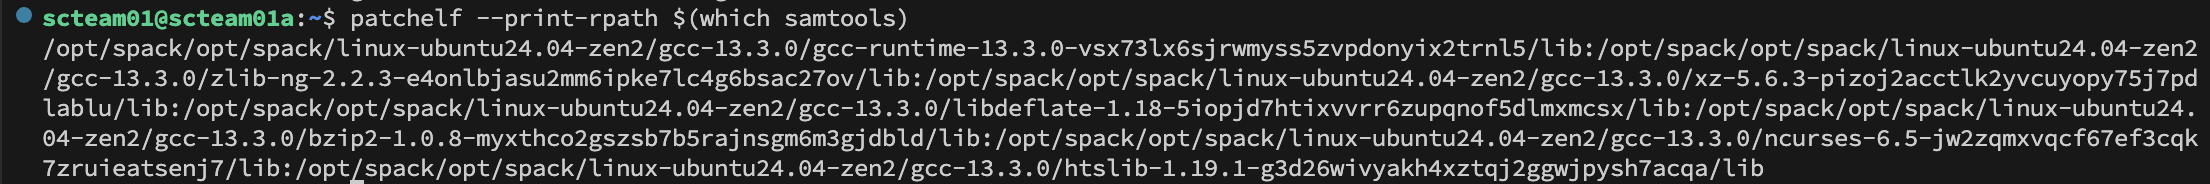
\includegraphics[width=1\textwidth]{./img/q2.png}
\end{center}

The output shows the RPATH of the Samtools executable.
\begin{lstlisting}[language=bash, basicstyle=\ttfamily\small, numbers=left, numberstyle=\tiny\color{gray}, stepnumber=1, frame=single, breaklines=true, breakatwhitespace=false]
/opt/spack/opt/spack/linux-ubuntu24.04-zen2/gcc-13.3.0/gcc-runtime-13.3.0-vsx73lx6sjrwmyss5zvpdonyix2trnl5/lib:/opt/spack/opt/spack/linux-ubuntu24.04-zen2/gcc-13.3.0/zlib-ng-2.2.3-e4onlbjasu2mm6ipke7lc4g6bsac27ov/lib:/opt/spack/opt/spack/linux-ubuntu24.04-zen2/gcc-13.3.0/xz-5.6.3-pizoj2acctlk2yvcuyopy75j7pdlablu/lib:/opt/spack/opt/spack/linux-ubuntu24.04-zen2/gcc-13.3.0/libdeflate-1.18-5iopjd7htixvvrr6zupqnof5dlmxmcsx/lib:/opt/spack/opt/spack/linux-ubuntu24.04-zen2/gcc-13.3.0/bzip2-1.0.8-myxthco2gszsb7b5rajnsgm6m3gjdbld/lib:/opt/spack/opt/spack/linux-ubuntu24.04-zen2/gcc-13.3.0/ncurses-6.5-jw2zqmxvqcf67ef3cqk7zruieatsenj7/lib:/opt/spack/opt/spack/linux-ubuntu24.04-zen2/gcc-13.3.0/htslib-1.19.1-g3d26wivyakh4xztqj2ggwjpysh7acqa/lib
\end{lstlisting}


\section*{Q3}
% Use LD_DEBUG to identify which curl library is being used by Samtools.

\begin{lstlisting}[language=bash, basicstyle=\ttfamily\small, numbers=left, numberstyle=\tiny\color{gray}, stepnumber=1, frame=single, breaklines=true, breakatwhitespace=false]
$ LD_DEBUG=libs samtools 2>&1 | grep curl
\end{lstlisting}

\begin{center}
    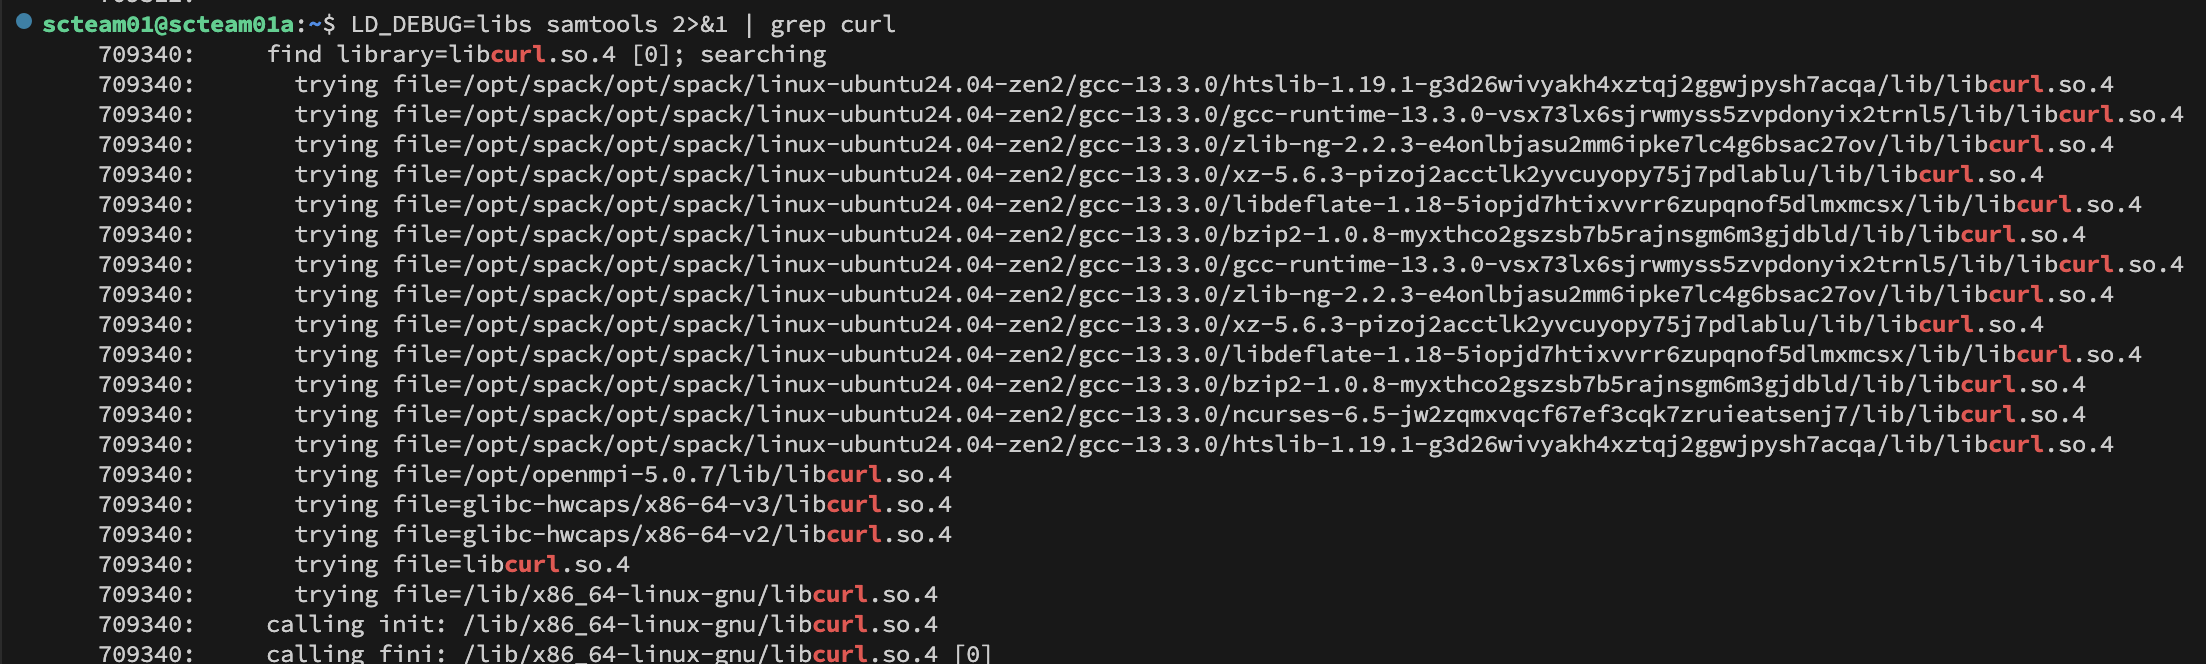
\includegraphics[width=1\textwidth]{./img/q3.png}
\end{center}

From the output, we found that the actual loaded path is:
\begin{lstlisting}[language=bash, basicstyle=\ttfamily\small, numbers=left, numberstyle=\tiny\color{gray}, stepnumber=1, frame=single, breaklines=true, breakatwhitespace=false]
/lib/x86_64-linux-gnu/libcurl.so.4
\end{lstlisting}

\section*{Q4}

\begin{center}
    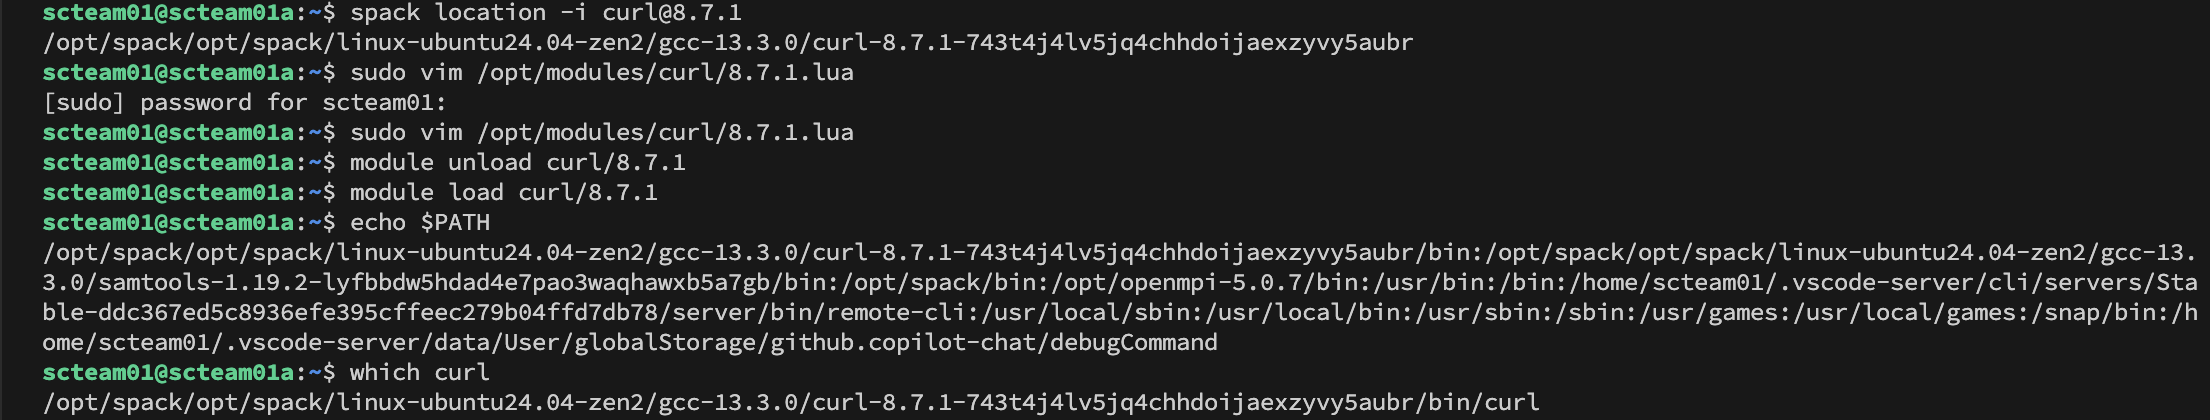
\includegraphics[width=1\textwidth]{./img/q4-1.png}
\end{center}

First, create a Lua-based Lmod modulefile for \texttt{curl@8.7.1}. When loaded, the module performs the following:

\begin{itemize}
  \item Adds the \texttt{bin} directory of \texttt{curl@8.7.1} to the \texttt{PATH}, allowing the \texttt{curl} command to be used directly from the terminal.
  \item Appends the \texttt{include} path to \texttt{CPATH} and the \texttt{lib} path to \texttt{LIBRARY\_PATH}, enabling static linking with \texttt{libcurl.a} and access to header files during compilation.
  \item Prepends the \texttt{lib} path to \texttt{LD\_LIBRARY\_PATH}, ensuring this version of \texttt{libcurl.so} has priority during dynamic linking.
\end{itemize}

Below are the commands used to install curl and create the module:

\begin{lstlisting}[language=bash, basicstyle=\ttfamily\small, numbers=left, numberstyle=\tiny\color{gray}, stepnumber=1, frame=single, breaklines=true, breakatwhitespace=false]
$ spack install --deprecated curl@8.7.1
$ spack location -i curl@8.7.1 # to find the installation path
$ sudo vim /opt/modules/curl/8.7.1.lua # to edit the module file
$ module use /opt/modules
$ module load curl/8.7.1
$ echo $PATH # to check if the module is loaded
$ which curl 
\end{lstlisting}

The output conforms that the correct version of curl is loaded:

\begin{lstlisting}[language=bash, basicstyle=\ttfamily\small, numbers=left, numberstyle=\tiny\color{gray}, stepnumber=1, frame=single, breaklines=true, breakatwhitespace=false]
/opt/spack/opt/spack/linux-ubuntu24.04-zen2/gcc-13.3.0/curl-8.7.1-743t4j4lv5jq4chhdoijaexzyvy5aubr/bin/curl
\end{lstlisting}

Below is the complete content of the \texttt{/opt/modules/curl/8.7.1.lua} modulefile:

\begin{center}
    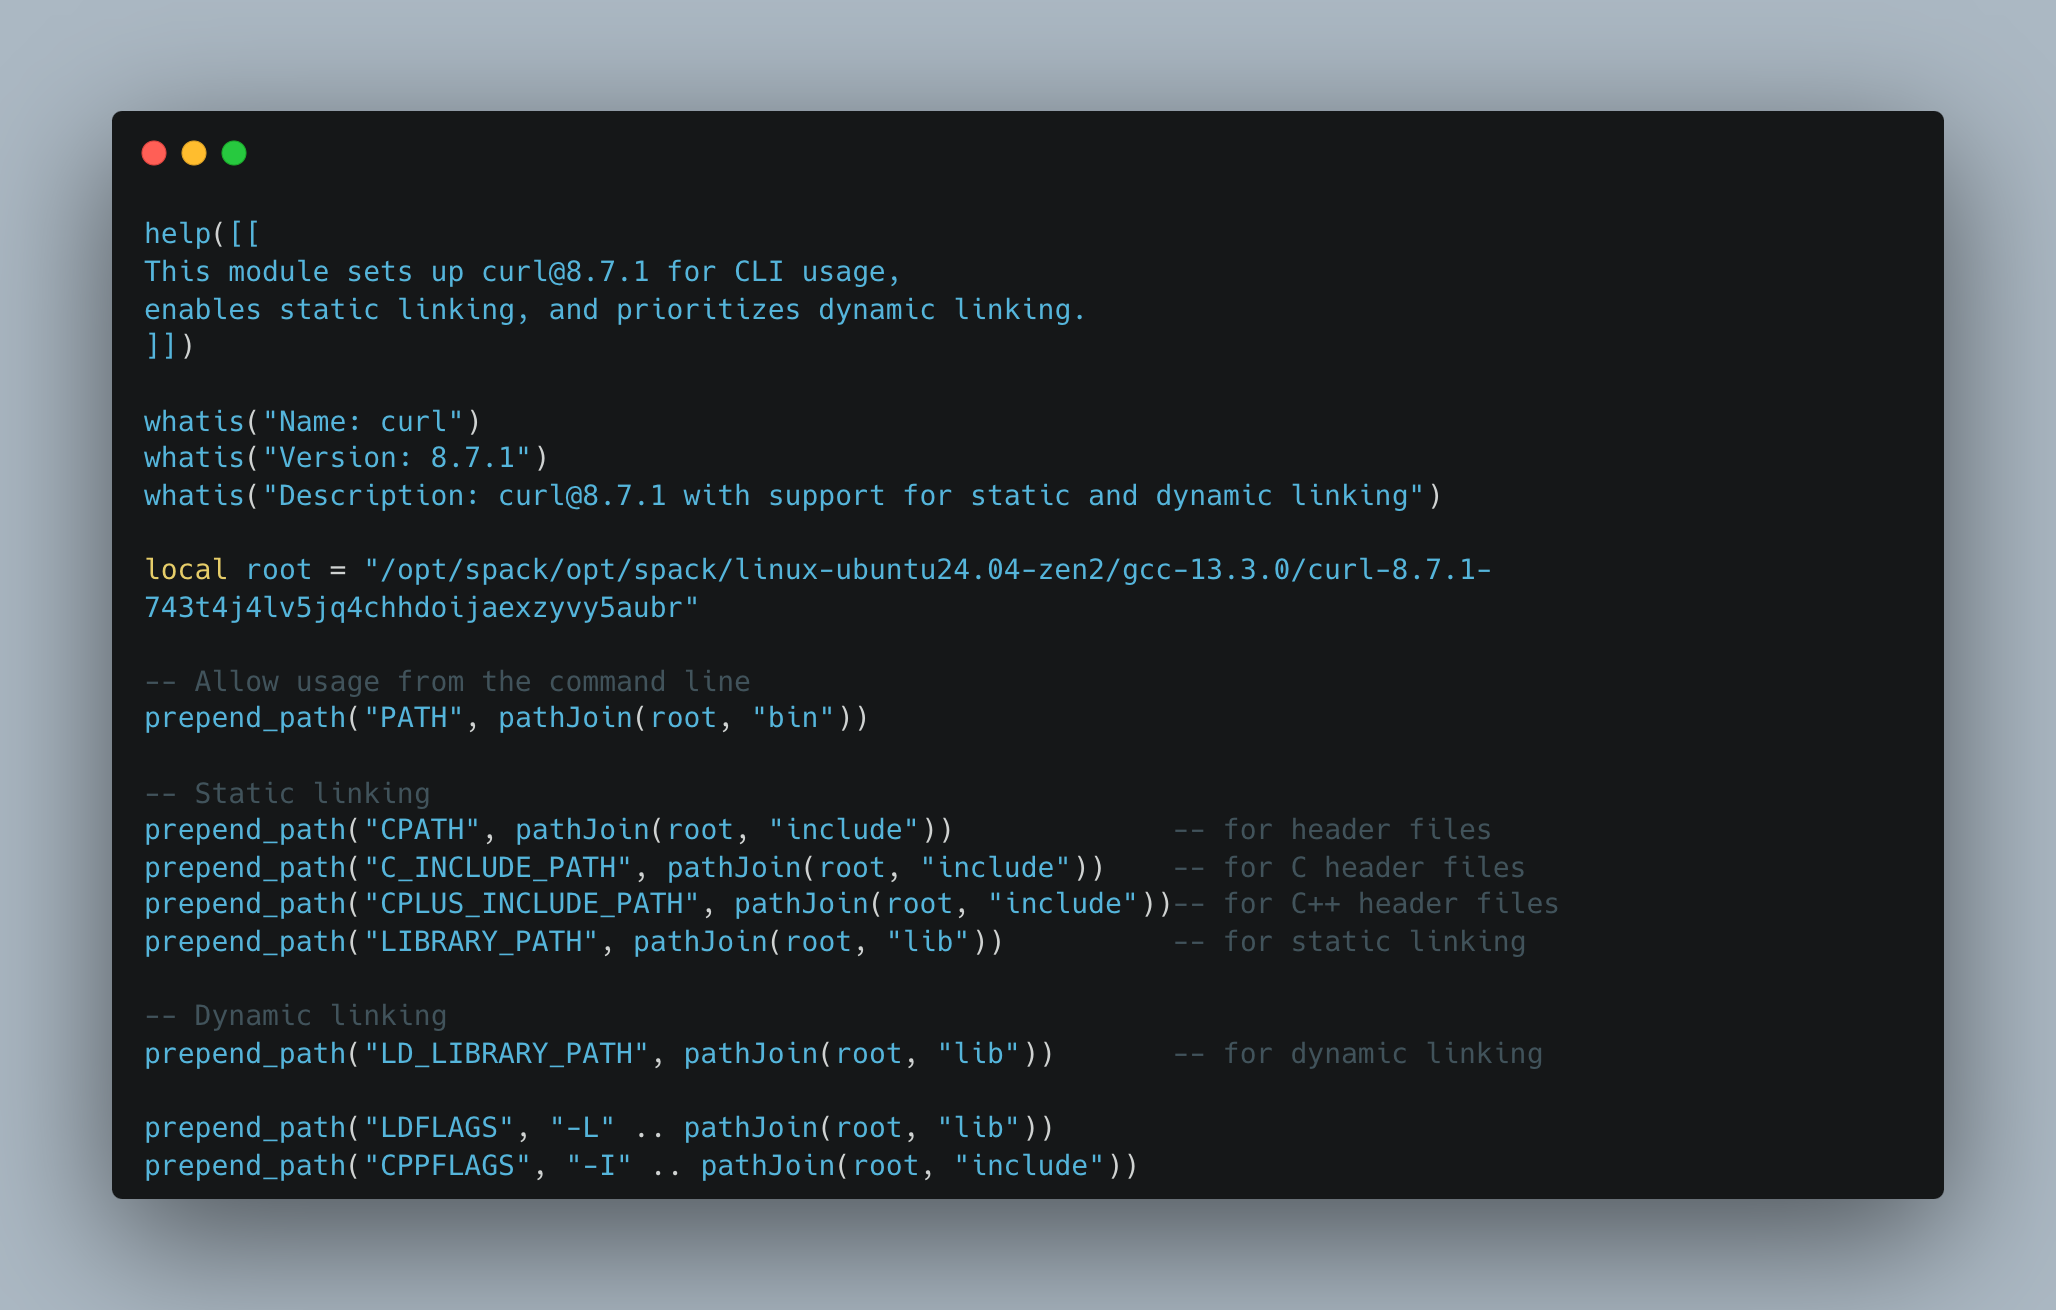
\includegraphics[width=1\textwidth]{./img/q4-2.png}
\end{center}

% \begin{lstlisting}[basicstyle=\ttfamily\small, frame=single, numbers=left, numberstyle=\tiny\color{gray}, stepnumber=1, breaklines=true, breakatwhitespace=false]
% help([[
% This module sets up curl@8.7.1 for CLI usage,
% enables static linking, and prioritizes dynamic linking.
% ]])

% whatis("Name: curl")
% whatis("Version: 8.7.1")
% whatis("Description: curl@8.7.1 with support for static and dynamic linking")

% local root = "/opt/spack/opt/spack/linux-ubuntu24.04-zen2/gcc-13.3.0/curl-8.7.1-743t4j4lv5jq4chhdoijaexzyvy5aubr"

% -- Allow usage from the command line
% prepend_path("PATH", pathJoin(root, "bin"))

% -- Static linking
% prepend_path("CPATH", pathJoin(root, "include"))             -- for header files
% prepend_path("C_INCLUDE_PATH", pathJoin(root, "include"))    -- for C header files
% prepend_path("CPLUS_INCLUDE_PATH", pathJoin(root, "include"))-- for C++ header files
% prepend_path("LIBRARY_PATH", pathJoin(root, "lib"))          -- for static linking

% -- Dynamic linking
% prepend_path("LD_LIBRARY_PATH", pathJoin(root, "lib"))       -- for dynamic linking

% prepend_path("LDFLAGS", "-L" .. pathJoin(root, "lib"))
% prepend_path("CPPFLAGS", "-I" .. pathJoin(root, "include"))
% \end{lstlisting}

\section*{Q5}

To remove the embedded \texttt{RPATH} from the Samtools binary, we can use the \texttt{patchelf} command.

\begin{lstlisting}[language=bash, basicstyle=\ttfamily\small, numbers=left, numberstyle=\tiny\color{gray}, stepnumber=1, frame=single, breaklines=true, breakatwhitespace=false]
$ patchelf --remove-rpath $(which samtools)
\end{lstlisting}

This command removes the RPATH from the Samtools executable. After executing this command, the \texttt{RPATH} will be empty.

\begin{lstlisting}[language=bash, basicstyle=\ttfamily\small, numbers=left, numberstyle=\tiny\color{gray}, stepnumber=1, frame=single, breaklines=true, breakatwhitespace=false]
$ patchelf --print-rpath $(which samtools)
(empty output)
\end{lstlisting}

\section*{Q6}
% Load the modulefile you wrote in Q4 and identify which curl library is currently being used by Samtools and explain why.

\begin{lstlisting}[language=bash, basicstyle=\ttfamily\small, numbers=left, numberstyle=\tiny\color{gray}, stepnumber=1, frame=single, breaklines=true, breakatwhitespace=false]
$ module load curl/8.7.1
$ LD_DEBUG=libs samtools 2>&1 | grep curl
\end{lstlisting}

The output showed:

\begin{lstlisting}[language=bash, basicstyle=\ttfamily\small, numbers=left, numberstyle=\tiny\color{gray}, stepnumber=1, frame=single, breaklines=true, breakatwhitespace=false]
...
calling init: /opt/spack/opt/spack/linux-ubuntu24.04-zen2/gcc-13.3.0/curl-8.7.1-743t4j4lv5jq4chhdoijaexzyvy5aubr/lib/libcurl.so.4
calling fini: /opt/spack/opt/spack/linux-ubuntu24.04-zen2/gcc-13.3.0/curl-8.7.1-743t4j4lv5jq4chhdoijaexzyvy5aubr/lib/libcurl.so.4 [0]
\end{lstlisting}

\begin{center}
    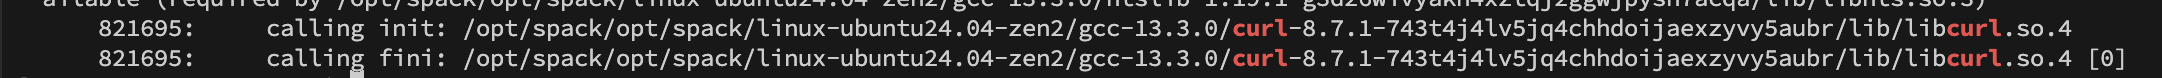
\includegraphics[width=1\textwidth]{./img/q6.png}
\end{center}

After loading our curl/8.7.1 module, Samtools is now using the Spack-installed curl library instead of the system one we saw in Q3. This happens because our module prepends the Spack curl library path to the LD\_LIBRARY\_PATH environment variable. The dynamic linker now searches directories in the LD\_LIBRARY\_PATH before looking in system directories, leading it to find and load our specified curl library first.


\end{document}
